\section{User Interaction Models}
\label{sec:interactive:models}

This section formally introduces \emph{Program Navigation} and \emph{Conversational Clarification} -- our proposed user
interaction models to improve the transparency of intent disambiguation process.
We have built a prototype UI called PROSE \FlashProg,\footnote{Available at
\url{https://prose-playground.cloudapp.net}.} which incorporates both interaction models, and used it to conduct a user
study.
In the study, we asked participants to extract structured data from semi-structured text files using \FlashProg.
We observe that participants perform more correct extraction when they
make use of the new interaction models.

To our surprise, participants preferred \ConversationalClarification over \ProgramNavigation slightly more even though
past case studies suggested that users wanted to look at the synthesized programs.
We believe this is explained by the fact that
because \ConversationalClarification is a \emph{proactive} interface that asks clarifying questions, whereas
\ProgramNavigation is a \emph{reactive} interface that expects an explicit correction of a mistake.

\subsection{User Interface}

\Cref{fig:interactive:ui:overview} shows a \FlashProg window after providing several examples (on the left), and after
invoking the learning process (on the right).
The \FlashProg window consists of 3 sections: \TopToolbarView (1), \InputTextView (2), and \PBEView (3).

\begin{figure}[p!]
    \centering
    \uwsinglespace
    \begin{tcbraster}[beamer, raster columns=1, size=minimal]
        \centering
        \tcbincludegraphics[scale=0.8]{figures/FlashProgMod4-before}
    \end{tcbraster}
    \vspace*{\baselineskip}
    \begin{tcbraster}[beamer, raster columns=1, size=minimal]
        \centering
        \tcbincludegraphics[scale=0.8]{figures/FlashProgMod4}
    \end{tcbraster}
    \caption{\FlashProg UI with PBE Interaction View in the ``Output'' mode, before and after the learning process.
        1 -- \TopToolbarView, 2 -- \InputTextView, 3 -- \PBEView.}
    \label{fig:interactive:ui:overview}
\end{figure}

% The \TopToolbarView contains: (a) an input button to open and upload files,
% (b) a button that resets \FlashProg to an initial state,
% (c) undo/redo buttons as expected,
% and (d) a ``Results'' button to download the output as a CSV file for further processing.

The \InputTextView is the main area.
It gives users the ability to provide examples by highlighting desired sections of the document, producing a set of
nested colored blocks.
Additionally, users may omit the structure boundary and only provide examples for the fields as shown in
\Cref{fig:interactive:ui:overview}.
After an automated learning phase, the output of the highest ranked program is displayed in the Output pane.
Each new row in the output is also matched to the corresponding region of the original document that is highlighted with
dimmer colors.
The user can also provide \emph{negative examples} by clicking on previously marked regions to communicate to the PBE
system that the region
should not be selected as part of the output.

The \PBEView is a tabbed pane giving users an opportunity to interact with the PBE system in three different ways: (i)
exploring the produced output,
(ii) exploring the learned program set paraphrased into English in the program viewer (\ProgramNavigation),
and (iii)~engaging in an active learning session through the ``Disambiguation'' feature
(\ConversationalClarification).\footnote{
    Note that throughout this chapter, I refer to the ``disambiguation'' as an overall problem of selecting the program
    that realizes user's intent in PBE.
    However, in our UI we use the word ``Disambiguation'' as a header of a pane with one iteration of the
    \ConversationalClarification process.
    We found that it describes \ConversationalClarification most lucidly to the users.
    % Hereinafter in the chapter, I refer to the ``Disambiguation pane'' in our UI
    % if the context does not facilitate any confusion with the ``disambiguation problem''.
}

The Output pane displays the current state of data extraction result either as a relational table or as a tree.
To facilitate exploration of the data, the \InputTextView is scrolled to
the source position of each cell when the user hovers over it.
The user can also mark incorrect table rows as negative examples.

\begin{figure}[t]
    \centering
    \uwsinglespace
    \begin{tcbraster}[beamer, raster columns=1, size=minimal]
        \centering
        \tcbincludegraphics[scale=0.6]{figures/paraphrasing}
    \end{tcbraster}
    \caption{\ProgramNavigationTab of the PROSE \FlashProg.
        It shows the extraction programs that were learned in the session in \Cref{fig:interactive:ui:overview}.
        They are paraphrased in English and indented.}
    \label{fig:interactive:ui:paraphrasing}
\end{figure}

\begin{figure}[t]
    \uwsinglespace
    \begin{tcbraster}[beamer, raster columns=1, size=minimal]
        \centering
        \tcbincludegraphics[scale=0.7]{figures/05-author-list-alternative-program}
    \end{tcbraster}
    \caption{\ProgramNavigationTab \& alternative subexpressions.}
    \label{fig:interactive:ui:alternatives}
\end{figure}

\begin{figure}[t]
    \begin{tcbraster}[beamer, raster columns=1, size=minimal]
        \centering
        \tcbincludegraphics[scale=0.7]{figures/07-author-disambiguation-full}
    \end{tcbraster}
    \caption{\ConversationalClarification being used to disambiguate different programs that extract individual
    authors.}
    \label{fig:interactive:ui:disambiguation}
\end{figure}

The Program viewer pane (\Cref{fig:interactive:ui:paraphrasing}) lets users explore the learned programs.
We concisely describe regexes that are used to match strings in the input text.
For instance, ``\texttt{Words/dots/hyphens $\concat$ WhiteSpace}''
represents \texttt{[-.\textbackslash p{Lu}\textbackslash  p{Ll}]+o\textbackslash p{Zs}+} (viewable in code mode).
To facilitate understanding of these regexes, when the user hovers over
part of a regex, our UI highlights matches of that part in the text.
In \Cref{fig:interactive:ui:paraphrasing}, \texttt{Name-Struct} refers to the region
between two consecutive names; \texttt{City-Struct} refers to the region
between \texttt{City} and the end of the enclosing \texttt{Name-Struct} region.
Learned programs reference these regions to extract data.
For instance, \texttt{Phone} is learnt relatively to enclosing
\texttt{City-struct} region: ``\texttt{second line}'' refers to the line in the \texttt{City} region.
In addition, clicking on the triangular marker opens a list of alternative suggestions for each subexpression.
We show number of highlights that will be added (or changed/removed) by the alternative
program as a +number (or a -number).
If the program is incorrect, the user can replace some expressions with alternatives from the suggested list
(\Cref{fig:interactive:ui:alternatives}).

The Disambiguation pane (\Cref{fig:interactive:ui:disambiguation}) presents the \ConversationalClarification interaction
model.
The PBE engine often learns multiple programs that are consistent with the examples but produce different outputs
on the rest of the document.
In such cases, this difference is highlighted and user is presented with an option to choose between the two behaviors.
Choosing one of the options is always equivalent to providing one more example (either positive or negative), thereby
invoking the learning again on the extended specification.

\subsection{\ProgramNavigation}
The two key challenges in \ProgramNavigation are: paraphrasing of the DSL programs in English, and providing alternative
suggestions for program expressions.

\paragraph{Templating language}
To enable paraphrasing, we implemented a high\hyp{}level templating language, which maps \emph{partial programs} into
\emph{partial English phrases}.
\citeauthor{pbd-fail} stated~\cite{pbd-fail}:
\begin{quote}
    \textit{``Users complained about arcane
        instructions such as ``set the \texttt{CharWeight} to $1$'' (make the text bold).
        $[\ldots]$ SMARTedit users also thought a higher-level description such as ``delete all
    hyperlinks'' would be more understandable than a series of lower level editing commands.''}
\end{quote}
Our template-based strategy for paraphrasing avoids arcane instructions by using \emph{context-sensitive formatting
rules}, and avoids low-level instructions by using \emph{idioms}, solving the aforementioned two
problems~\cite{flashprog}.

\paragraph{Program alternatives}
To enable alternatives, we record the original candidate program set for each subexpression in the chosen program.
Since it is represented as a VSA, we can easily retrieve a subspace of alternatives for each program subexpression, and
apply the domain-specific ranking function on them.
The top $5$ alternatives are presented to the user.

\subsection{\ConversationalClarification}
\ConversationalClarification selects examples based on different outputs produced by generated programs.
Each synthesis step produces a VSA of ambiguous programs that are consistent with the given examples.
\ConversationalClarification iteratively replaces the subexpressions of the top-ranked program with its top $k$
alternatives from the VSA.
The clarifying question for the user is based on the \emph{first discrepancy} between the outputs of the currently
selected program $P$ and an alternative program $P'$.
Such a discrepancy can have three possible manifestations:
\begin{itemize}[nosep]
    \item The outputs of $P$ and $P'$ match until $P$ selects a region $r$, which does not intersect any selection of
        $P'$.
        This leads to the question ``Should $r$ be highlighted or not?''
    \item The outputs of $P$ and $P'$ match until $P'$ selects a region $r'$, which does not intersect any selection of
        $P$.
        This leads to the question ``Should $r'$ have been highlighted?''
    \item The outputs of $P$ and $P'$ match until $P$ selects a region $r$, $P'$ selects a different region $r'$, and
        $r$ intersects
        $r'$.
        This leads to the question ``Should $r$ or $r'$ be highlighted?''
\end{itemize}
For better usability (and faster convergence), we merge the three question types into
one, and ask the user ``What should be highlighted: $r_1$, $r_2$, or nothing?''
Selecting $r_1$ or $r_2$ would mark the selected region as a positive example.
Selecting ``nothing'' would mark both $r_1$ and $r_2$ as negative examples.
After selecting an option, we convert the choice into one or more examples, and invoke a new synthesis process.

\subsection{Evaluation}
\newcommand{\plural}[3]{\ifnum 1=#1 #1 #2\xspace\else #1 #3\xspace\fi}
\newcommand{\ifequal}[4]{\ifnum #1=#2 #3\else #4\fi}

\newcommand{\numPeopleSurvey}{29}
\newcommand{\numPeopleOptin}{80}
\newcommand{\numPeopleEarlyTesters}{4}
\newcommand{\numWomen}{4}
\newcommand{\numMen}{25}
\newcommand{\minAge}{19}
\newcommand{\maxAge}{34}
\newcommand{\minProgrammingExperienceYears}{0}
\newcommand{\maxProgrammingExperienceYears}{less than 20 years}
\newcommand{\minDataExtractionFrequency}{never or several times a year}
\newcommand{\maxDataExtractionFrequency}{every day}
\newcommand{\percentagePreferenceFlashProg}{72}
\newcommand{\recommendFlashProgPercentage}{100}
\newcommand{\excitementPercentToHaveFlashProgFourOrFive}{79}
\newcommand{\percentageUsingProgramViewer}{45}
\newcommand{\percentageUsingDisambiguation}{93}
\newcommand{\usefulnessProgramViewer}{4.2}
\newcommand{\usefulnessProgramViewerStdDev}{2.12}
\newcommand{\usefulnessDisambiguation}{5.4}
\newcommand{\usefulnessDisambiguationStdDev}{1.50}
\newcommand{\numUserPreferringProgramViewer}{4}
\newcommand{\numUserPreferringDisambiguation}{15}
\newcommand{\numUserUsingDisambiguation}{27}
\newcommand{\numPeopleAlwaysOrAlmostAlwaysCorrectDisambiguation}{17}
\newcommand{\numPeopleNotAlwaysCorrectDisambiguation}{10}
\newcommand{\numPeopleOtherCorrectDTFirstLastTask}{0}
\newcommand{\numUsersProgramNavigation}{13}
\newcommand{\numUsersProgramNavigationHighlightingHardToUse}{1}
\newcommand{\numUsersProgramNavigationHighlightingNaturalLoved}{6}
\newcommand{\numInputTextViewUsefulSeven}{22}
\newcommand{\numInputTextViewUsefulSix}{5}
\newcommand{\numInputTextViewUsefulFiveOrLess}{2}
\newcommand{\inputTextViewUsefulnessSixOrSeven}{96}
\newcommand{\disambiguationCorrectnessTaskOne}{(3, 5) (0, 4) (5, 3) (0, 2) (0, 1)}
\newcommand{\disambiguationCorrectnessTaskTwo}{(4, 5) (3, 4) (0, 3) (1, 2) (0, 1)}
\newcommand{\disambiguationCorrectnessTaskThree}{(4, 5) (3, 4) (2, 3) (2, 2) (0, 1)}
\newcommand{\excitementPercentToHaveFlashProgFive}{8}
\newcommand{\excitementPercentToHaveFlashProgFour}{15}
\newcommand{\excitementPercentToHaveFlashProgThree}{6}
\newcommand{\preferredToHaveFlashProgFive}{4}
\newcommand{\preferredToHaveFlashProgFour}{17}
\newcommand{\preferredToHaveFlashProgThree}{3}
\newcommand{\preferredToHaveFlashProgTwoOrLess}{4}
\newcommand{\percentageUsefulTextViewSevenOrSix}{93}
\newcommand{\usefulnessDisambiguationTaskOne}{(3, 7) (1, 6) (3, 5) (1, 4) (1, 3) (0, 2) (0, 1)}
\newcommand{\usefulnessDisambiguationTaskTwo}{(3, 7) (2, 6) (2, 5) (1, 4) (0, 3) (0, 2) (0, 1)}
\newcommand{\usefulnessDisambiguationTaskThree}{(3, 7) (3, 6) (3, 5) (1, 4) (1, 3) (0, 2) (1, 1)}
\newcommand{\usefulnessProgramViewerTaskOne}{(1, 7) (1, 6) (1, 5) (1, 4) (0, 3) (1, 2) (3, 1)}
\newcommand{\usefulnessProgramViewerTaskTwo}{(3, 7) (1, 6) (2, 5) (1, 4) (2, 3) (2, 2) (1, 1)}
\newcommand{\usefulnessProgramViewerTaskThree}{(2, 7) (1, 6) (2, 5) (1, 4) (2, 3) (1, 2) (0, 1)}
\newcommand{\appreciationRegExpHighlightingTaskOne}{(1, 4) (1, 3) (0, 2) (1, 1)}
\newcommand{\appreciationRegExpHighlightingTaskTwo}{(0, 4) (1, 3) (2, 2) (0, 1)}
\newcommand{\appreciationRegExpHighlightingTaskThree}{(1, 4) (2, 3) (2, 2) (0, 1)}
\newcommand{\numPeopleNotUsingSuggestionViewer}{9}
\newcommand{\numKnowledgeablePeoplePreferringDisambiguation}{7}
%NEWCOMMANDS

\newcommand{\BI}{BI\xspace}
\newcommand{\BIdef}{Basic Interface\xspace}

\newcommand{\BIPW}{BI + \ProgramNavigationInitials\xspace}
\newcommand{\BIPWdef}{\BI + \ProgramNavigation\xspace}

\newcommand{\BIDT}{BI + \ConversationalClarificationInitials\xspace}
\newcommand{\BIDTdef}{\BI + \ConversationalClarification\xspace}

\newlength{\xdim}

\newcommand{\maxusersgraphs}{10} % Used in the usefulness graphs

\definecolor{NumUserColor}{HTML}{1C19D7}
\definecolor{NumTaskOne}{HTML}{E3EA8B}
\definecolor{NumTaskTwo}{HTML}{C3BFFB}
\definecolor{NumTaskThree}{HTML}{639A2B}




To evaluate the usefulness of our novel interaction models for disambiguation, we conducted a user study in the data
wrangling domain.
In particular, we address three research questions for PBE:
\newcommand{\RQOneShort}{RQ1}
\newcommand{\RQTwoShort}{RQ2}
\newcommand{\RQThreeShort}{RQ3}
\newcommand{\RQOne}{Do \ProgramNavigation and \ConversationalClarification contribute to correctness?}
\newcommand{\RQTwo}{Which of \ProgramNavigation and \ConversationalClarification is perceived more useful for data extraction?}
\newcommand{\RQThree}{Do our novel interaction models help alleviate typical distrust in PBE systems?}
\begin{itemize}[nosep]
    \item \RQOneShort: \RQOne
    \item \RQTwoShort: \RQTwo
    \item \RQThreeShort: \RQThree
\end{itemize}

\paragraph{User study design}
Because typical data wrangling tasks can be solved without any programming skills, we performed a
within-subject study over an heterogeneous population of \numPeopleSurvey{} people: \plural{\numWomen}{woman}{women}
aged between 19 and 24 and \plural{\numMen}{man}{men} aged between \minAge{} and \maxAge{}.
Their programming experience ranged from none (a 32-year man doing extraction tasks several
times a month), less than~5~years~(8 people), less than~10~(9), less than~15~(8) to less than 20~(3).
They reported performing data extraction tasks never (4 people), several times a year (7),
several times a month (11), several times a week (3) up to every day~(2).

We selected 3 files containing several ambiguities these users have to find out and to resolve.
We chose these files among anonymized files provided by our customers.
Our choice was also motivated by repetitive tasks, where extraction programs are meant to be
reused on other similar files.
The three files are the following:
\todoinline{Add additional figures.}

\newcommand{\BankListing}{Bank listing}
\newcommand{\AmazonListing}{Amazon research}
\newcommand{\HydrogensListing}{Bioinformatic log}
\begin{description}[nosep]
    \item[1. \BankListing.] List of bank addresses and capital grouped by state.
        The postal code can be ambiguous.
    \item[2. Amazon research.] The text of the search results on Amazon for the query ``chair''.
        The data is visually structured as a list of records, but contains spacing and noise.
    \item[3. Bioinformatic log.] A log of numerical values obtained from five experiments, from bioinformatics
        research (\Cref{fig:interactive:evaluation:biosample,fig:interactive:evaluation:highlighting}).
        % A straightforward extraction misses one experiment.
\end{description}

\begin{figure}[t]
    \centering
    \includegraphics[width=0.6\columnwidth]{figures/hinthydrogens}
    \caption{Bioinformatic log: Result sample.}
    \label{fig:interactive:evaluation:biosample}
\end{figure}

\begin{figure}[t]
    \centering
    \includegraphics[width=0.7\columnwidth]{figures/hydrogenhybrid}
    \caption{Highlighting in the \InputTextView for obtaining~\Cref{fig:interactive:evaluation:biosample}.}
    \label{fig:interactive:evaluation:highlighting}
\end{figure}

After a brief tutorial, we ask users to perform extraction on the three files.
In order to measure the trust they give to the extraction, we do not tell them if their extraction is correct or not.
For each extraction task, we provide a result sample (such as \Cref{fig:interactive:evaluation:biosample}).
Users then manipulate \FlashProg to generate the entire output table corresponding to that task.

To answer \RQOneShort, we select a number of representative values across all fields
for each task, and we automatically measure how many of them were incorrectly highlighted.
These values were selected by running \FlashProg sessions in advance
ourselves and observing insightful checkpoints that require attention.
In total, we selected 6 values for task \#1, 13 for task \#2 and 12 for task \#3.
We do not notify users about their errors.
This metric has more meaning than if we recorded all errors.
As an illustration, a raw error measurement in the third task for a user forgetting about the third main record would
yield more than 140 errors.
Our approach returns 2 errors, one for the missing record, and one for another ambiguity that needed to be checked but
could not.
This makes error measurement comparable across tasks.

To measure the impact of \ProgramNavigation and \ConversationalClarification interaction models
independently, we set up three interface environments:

\begin{description}
    \item[\BIdef (\BI).] This environment enables only the PBE interaction model.
        It includes the following UI features: the labeling interface for mouse-triggered highlighting, the
        label menu to rename labels, to switch between them and the \OutputTab.
    \item[\BIPWdef (\BIPW).] Besides PBE, this interface enables the
        \ProgramNavigation interaction model, which includes the \ProgramNavigationTab and its features.
    \item[\BIDTdef (\BIDT).] Besides PBE, this environment enables the
        \ConversationalClarification interaction model, which includes the \ConversationalClarificationTab.
\end{description}

To compensate the learning curve effects when comparing the usefulness of various interaction models, we set up the
environments in three configurations A, B, and~C, shown in \Cref{tbl:playground:configurations}.
Each configuration has the same order of files/tasks, but we chose three environment permutations.
As we could not force people to finish the study, the number of users per environment is not perfectly balanced.

\begin{table}
    \centering
    \begin{tabular}{llllr} \toprule
        & \multicolumn{3}{c}{\textbf{Tasks}} & \\ \cmidrule(r){2-4}
        \multicolumn{1}{l}{\textbf{Configuration}} & \textbf{1. Bank} & \textbf{2. Amazon} & \textbf{3. Bio log} & \textbf{\# of users} \\ \midrule
        \multicolumn{1}{l}{\textbf{A}} & \BIPW & \BIDT & \multicolumn{1}{l}{\BI} & 8 \\
        \multicolumn{1}{l}{\textbf{B}} & \BI & \BIPW & \multicolumn{1}{l}{\BIDT} & 12 \\
        \multicolumn{1}{l}{\textbf{C}} & \BIDT & \BI & \multicolumn{1}{l}{\BIPW} & 9\\ \bottomrule
    \end{tabular}
    \caption{Configurations of the user study of user interaction models in \FlashProg.}
    \label{tbl:playground:configurations}
\end{table}

To answer \RQTwoShort{} and \RQThreeShort{}, we asked the participants about the
perceived usefulness of our novel interaction models, and the confidence
about the extraction of each file, using a Likert scale from 1 to 7, 1 being the
least useful/confident:

\begin{enumerate}[nosep]
    \item How confident were you in the final extraction result?
    \item After training, would you trust \FlashProg to work correctly on another similar file if you do not provide any
        examples?
    \item How easy was it for you to complete this task?
\end{enumerate}

\paragraph{Results}
We analyzed the data both from the logs collected by the UI instrumentation, and from the initial and final surveys.
% If a feature was activated, we counted the user for statistics even if he reported not using it.

\begin{figure}[t]
    \centering
    \includegraphics[width=0.6\columnwidth]{figures/error-plot1}
    \uwsinglespace
    \caption{Distribution of error counts across the three environments in the user study of data wrangling in
        \FlashProg.
        Both \ConversationalClarification{} (\ConversationalClarificationInitials) and
        \ProgramNavigation{} (\ProgramNavigationInitials) significantly decrease the number of errors.}
    \label{fig:interactive:study:errorcounts}
\end{figure}

\subsubsection*{\RQOneShort: \RQOne}
\textbf{Yes. We have found significant
reduction of number of errors with each of these new interaction models} (see \Cref{fig:interactive:study:errorcounts}).
Our new interaction models reduce the error rate in data extraction without any
negative effect on the users' extraction speed. To obtain this result, we applied the
Wilcoxon rank-sum test on the instrumentation data.
More precisely, users in \BIDT ($W=78.5$, $p=0.01$) and \BIPW ($W= 99.5$, $p=0.06$)
performed better than \BI, with no significant
difference between the two of them ($W=94$, \textit{n.s.}).
There was also no statistically significant difference between the completion time in \BI and
completion time in \BIDT ($W=178.5$, \textit{n.s.}) or \BIPW{} ($W=173$, \textit{n.s.}).

\subsubsection*{\RQTwoShort: \RQTwo}
\textbf{\ConversationalClarification is perceived more useful than \ProgramNavigation} (see
\Cref{fig:interactive:study:disambiguationuseful,fig:interactive:study:programnavigationuseful}).
Comparing the user-reported usefulness between the \ConversationalClarification and the \ProgramNavigation, on a
scale from 1 (not useful at all) to 7 (extremely useful), the
\ConversationalClarification has a mean score of \usefulnessDisambiguation{} ($\sigma =$
\usefulnessDisambiguationStdDev{})
whereas the \ProgramNavigation has \usefulnessProgramViewer{} ($\sigma =$ \usefulnessProgramViewerStdDev{})
Only \ifequal{\numUserPreferringProgramViewer}{1}{one user}{\numUserPreferringProgramViewer{} users} out of
\numPeopleSurvey{}
\ifequal{\numUserPreferringProgramViewer}{1}{scores}{score} \ProgramNavigation more useful than
\ConversationalClarification,
whereas \ConversationalClarification is scored more useful by
\numUserPreferringDisambiguation~\ifequal{\numUserPreferringDisambiguation}{1}{user}{users}.

\begin{figure}[t!]
    \centering
    \begin{subfigure}{\columnwidth}
        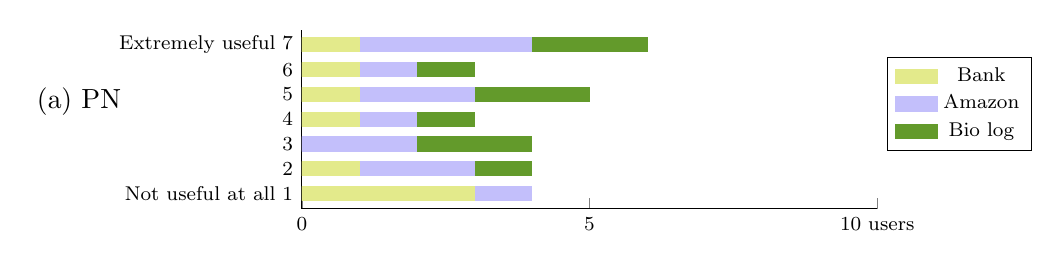
\begin{tikzpicture}[thick,scale=0.9]
            \begin{axis}[
                xbar stacked,
                legend style={
                    legend columns=1,
                    at={(0.85\columnwidth,0.05\columnwidth)},
                    anchor=south east
                },
                ytick=data,
                axis y line*=none,
                axis x line*=bottom,
                tick label style={font=\footnotesize},
                legend style={font=\footnotesize},
                label style={font=\footnotesize},
                xtick={0,5,10},
                xticklabels={0,5,10 users},
                width=.8\columnwidth,
                bar width=2mm,
                yticklabels={Extremely useful 7, 6, 5, 4, 3, 2, Not useful at all 1},
                xmin=0,
                xmax=\maxusersgraphs,
                area legend,
                y=3.5mm,
                ]
                \addplot[NumTaskOne,fill=NumTaskOne] coordinates
                    {\usefulnessProgramViewerTaskOne};
                \addplot[NumTaskTwo,fill=NumTaskTwo] coordinates
                    {\usefulnessProgramViewerTaskTwo};
                \addplot[NumTaskThree,fill=NumTaskThree] coordinates
                    {\usefulnessProgramViewerTaskThree};
                \legend{Bank, Amazon, Bio log};
            \coordinate (C) at (-31mm,11mm);
        \end{axis}
        \node at (C) {(a) PN};
    \end{tikzpicture}
    \phantomcaption
    \label{fig:interactive:study:disambiguationuseful}
\end{subfigure}
\begin{subfigure}{\columnwidth}
    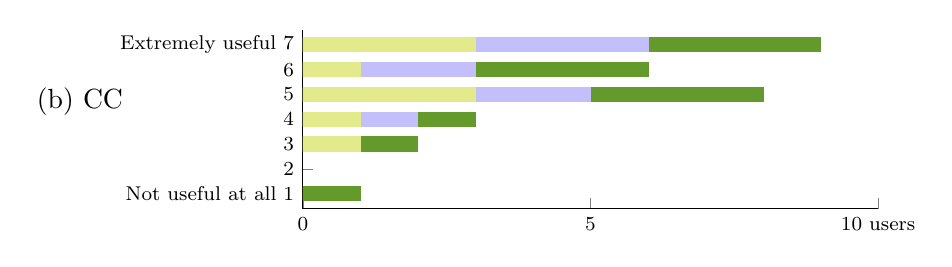
\begin{tikzpicture}[thick,scale=0.9]
        \begin{axis}[
            xbar stacked,
            legend style={
                legend columns=3,
                at={(xticklabel cs:0.5)},
                anchor=north,
                draw=none
            },
            ytick=data,
            axis y line*=none,
            axis x line*=bottom,
            tick label style={font=\footnotesize},
            legend style={font=\footnotesize},
            label style={font=\footnotesize},
            xtick={0,5,10},
            xticklabels={0,5,10 users},
            width=.8\columnwidth,
            bar width=2mm,
            yticklabels={Extremely useful 7, 6, 5, 4, 3, 2, Not useful at all 1},
            xmin=0,
            xmax=\maxusersgraphs,
            area legend,
            y=3.5mm,
            ]
            \addplot[NumTaskOne,fill=NumTaskOne] coordinates
                {\usefulnessDisambiguationTaskOne};
            \addplot[NumTaskTwo,fill=NumTaskTwo] coordinates
                {\usefulnessDisambiguationTaskTwo};
            \addplot[NumTaskThree,fill=NumTaskThree] coordinates
                {\usefulnessDisambiguationTaskThree};
            % \legend{Task 1, Task 2, Task 3}
            \coordinate (A) at (-31mm,11mm);
        \end{axis}
        \node at (A) {(b) CC};
    \end{tikzpicture}
    \phantomcaption
    \label{fig:interactive:study:programnavigationuseful}
\end{subfigure}
\begin{subfigure}{\columnwidth}
    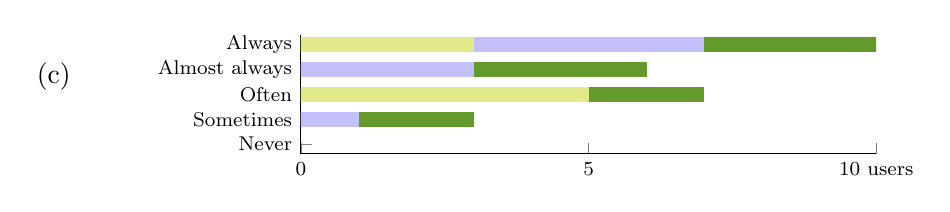
\begin{tikzpicture}[thick,scale=0.9]
        \begin{axis}[
            xbar stacked,
            legend style={
                legend columns=3,
                at={(xticklabel cs:0.5)},
                anchor=north,
                draw=none,
                draw=none
            },
            ytick=data,
            axis y line*=none,
            axis x line*=bottom,
            tick label style={font=\footnotesize},
            legend style={font=\footnotesize},
            label style={font=\footnotesize},
            xtick={0,5,10},
            xticklabels={0,5,10 users},
            width=.8\columnwidth,
            bar width=2mm,
            yticklabels={\phantom{Extremely} Always, Almost always, Often, Sometimes, Never},
            xmin=0,
            xmax=\maxusersgraphs,
            area legend,
            y=3.5mm,
            ]
            \addplot[NumTaskOne,fill=NumTaskOne] coordinates
                {\disambiguationCorrectnessTaskOne};
            \addplot[NumTaskTwo,fill=NumTaskTwo] coordinates
                {\disambiguationCorrectnessTaskTwo};
            \addplot[NumTaskThree,fill=NumTaskThree] coordinates
                {\disambiguationCorrectnessTaskThree};
            \coordinate (E) at (-34mm,8mm);
        \end{axis}
        \node at (E) {(c)};
    \end{tikzpicture}
    \phantomcaption
    \label{fig:interactive:study:disambiguationcorrect}
\end{subfigure}
\caption{User-reported: \textbf{(a)} usefulness of \ProgramNavigation, \textbf{(b)} usefulness of
    \ConversationalClarification, \textbf{(c)} correctness of one of the choices of \ConversationalClarification.}
\end{figure}

\subsubsection*{\RQThreeShort: \RQThree}
\textbf{Yes for \ConversationalClarification.}
The tasks finished with \ConversationalClarification
obtained a higher confidence score compared to those without ($W=181.5$, $p = 0.07$).
No significant difference was found for \ProgramNavigation ($W=152.5$, \textit{n.s.}).
Regarding the trust our users would have if they ran the learned program on
other data, we did not find any significant differences for
\ConversationalClarification ($W=146$, \textit{n.s.}) and \ProgramNavigation ($W=161$, \textit{n.s.}) over only \BI.

Regarding the question ``How often would you use \FlashProg, compared to
other extraction tools?'', on a Likert scale from 1 (never) to 5 (always), \preferredToHaveFlashProgFive{} users
answered 5, \preferredToHaveFlashProgFour{} answered 4, \preferredToHaveFlashProgThree{} answered 3, and the remaining
\preferredToHaveFlashProgTwoOrLess{} answered 2 or less.
Furthermore, \ifequal{\recommendFlashProgPercentage}{100}{all}{\recommendFlashProgPercentage\% of our users} would
recommend \FlashProg to others.
When asked how excited would they be to have such a tool on a scale from 1 to 5, \excitementPercentToHaveFlashProgFive{}
users answered~5, and \excitementPercentToHaveFlashProgFour{} answered 4.

The users' trust is supported by data: Perceived correctness is negatively correlated
with number of errors (Spearman $\rho=-0.25$, $p=0.07$).
Although we asked them to make sure the extraction is correct
and never told them they did errors, users making more errors  (thus unseen)
reported to be less sure about the extraction.
However, there is no significant correlation between number of errors made and
the programming experience mapped between 0 and 4 ($\rho=-0.09$, \textit{n.s.}).

\subsection{Conclusion}
The two key takeaways of this user study is that
\textbf{(a)} any user interaction model (\ProgramNavigation or \ConversationalClarification) reduces the number of
errors in the completed tasks and improves the users' confidence in the results (as compared to example-only workflow);
\textbf{(b)} \ConversationalClarification is perceived as more useful thanks to its proactivity and clarity.
Based on these observations, PROSE now includes a more general version of \ConversationalClarification (called
\emph{feedback-based synthesis}) as a key capability for any DSL.
The next section presents its design and applications.
